\section{Raw Data Reconstruction}\label{sec:data.cook}

The process of reconstructing tracks and their subsequent particle identification from raw data is referred to as ``cooking'' and was done by the program \texttt{a1c}\label{abbr:a1c} for \g12. ``Cooking'' is when the information recorded from the various detector subsystems is converted into a form suitable for physics analysis. During cooking, each detector subsystem was calibrated. The ``cooking'' of the \g12 dataset was performed by John Theodore Goetz and is fully documented in~\cite{clas.g12.note} and~\cite{goetz}.

The ``cooking'' process performed by \texttt{a1c} is outlined in Fig.~\ref{fig:data.cook.flowchart}. Initial calibrations are done for each subsystem in each sector the process begins with ``hit-based'' tracking in the \abbr{DC}. ``Hit-based'' tracking requires only the positions of wires registering a hit in a given sector. Adjacent hits in each superlayer are assembled into clusters, and then these clusters are linked in each region to produce track segments. Refer to Fig.~\ref{fig:clas.dc.drift} for an illustration of a track segment. Track segments are linked over the three regions to produce full hit-based trajectories. See Fig~\ref{fig:data.cook.flowchart.hitbased} for a pictorial description of ``hit-based'' tracking. There was an overall failure of events that should have passed ``hit-based'' tracking but failed. This will be discussed fully in Sec.~\ref{sec:analysis.accept.verify}.
%, but can be seen in Fig.~\ref{sec:clas.st.eff} as an overall inefficiency of 3.75\%.

\begin{figure}\begin{center}
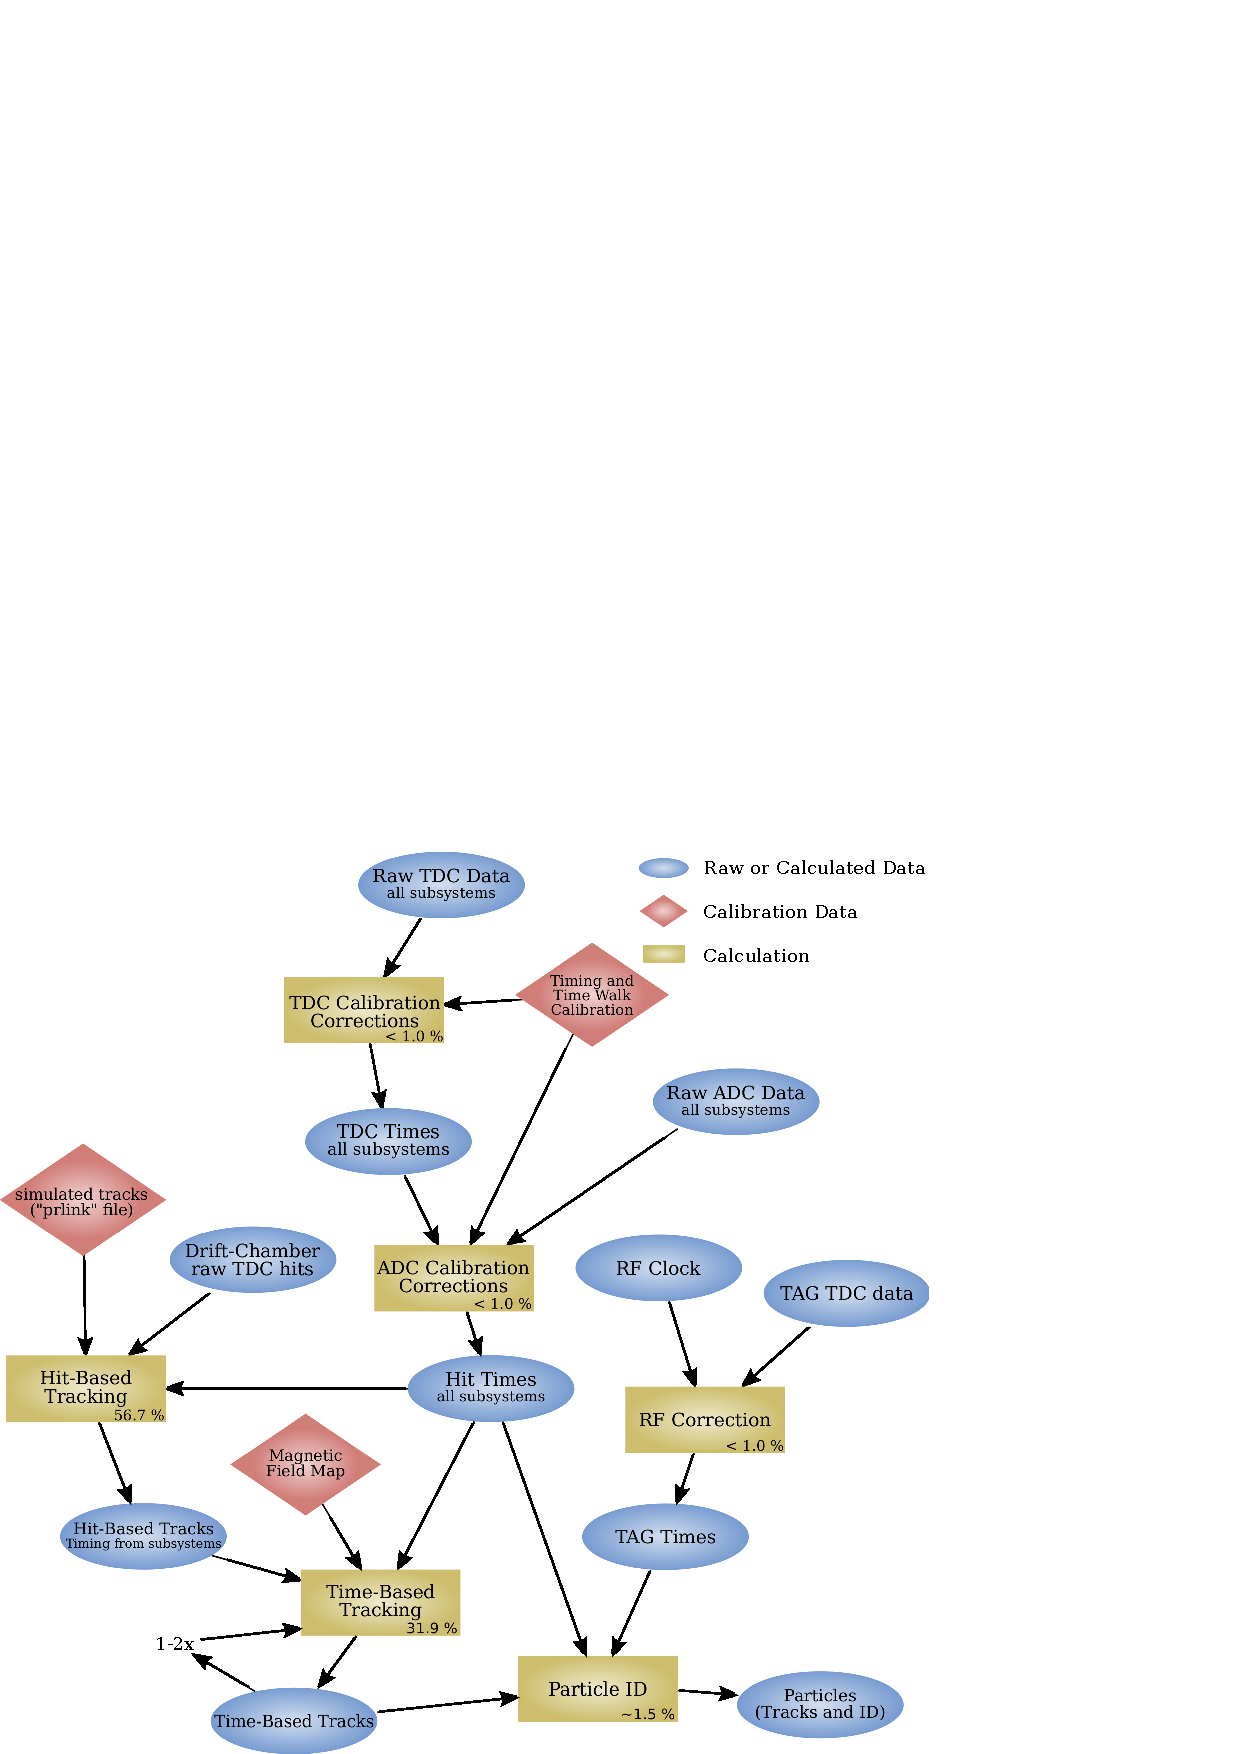
\includegraphics[width=0.92\columnwidth]{\figures/reconstruction/clas6_cooking_diagram_color.pdf}
\caption[Flow chart of the reconstruction process from raw data to identified tracks with momentum]{\label{fig:data.cook.flowchart}Flow chart of the reconstruction process from raw data to identified tracks with momentum. ``Subsystems'' refers to the \abbr{ST}, \abbr{CC}, \abbr{TOF} and the \abbr{EC} detectors. Percentages shown indicate the relative time taken to do the calculations.}
\end{center}\end{figure}

\begin{figure}\begin{center}
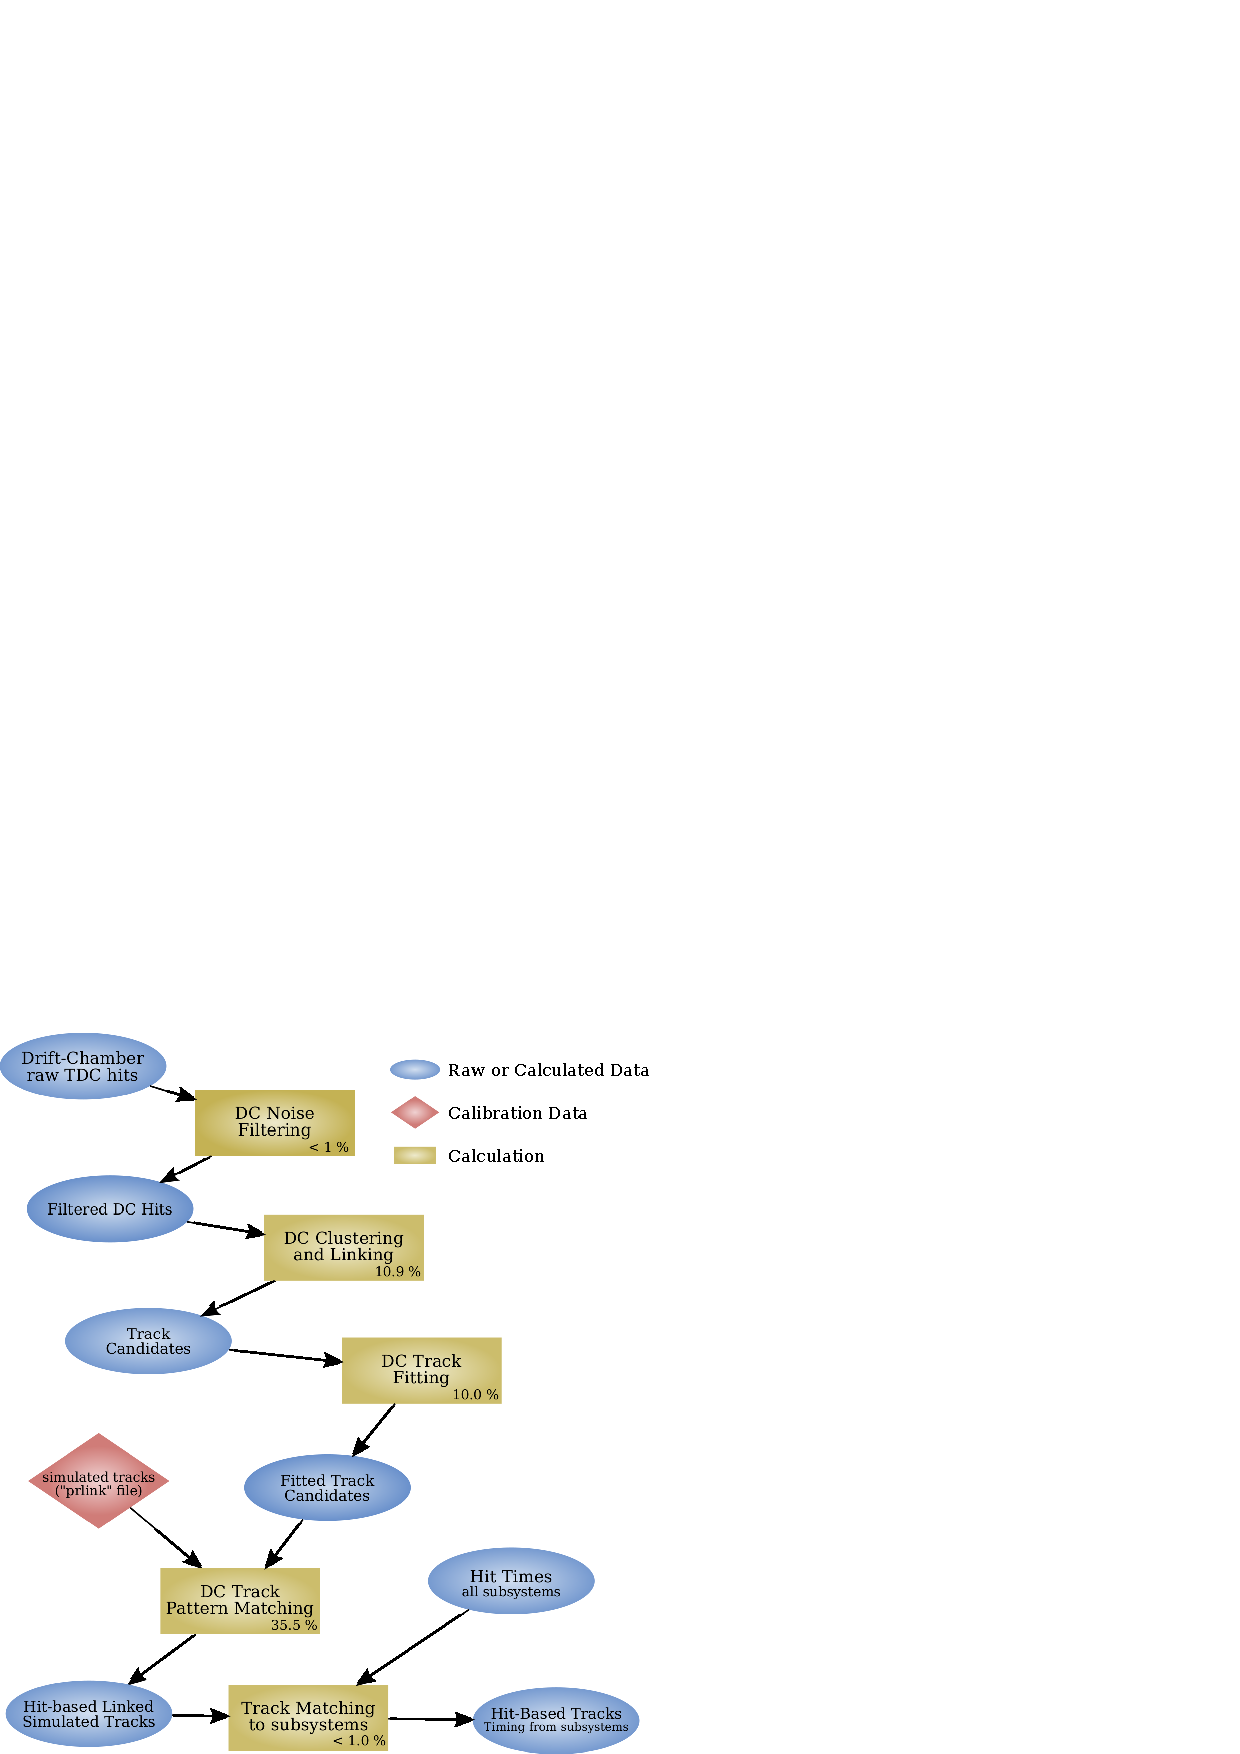
\includegraphics[width=0.7\columnwidth]{\figures/reconstruction/clas6_hitbasedtracking_diagram_color.pdf}
\caption[Flow chart of the hit-based tracking part of the reconstruction]{\label{fig:data.cook.flowchart.hitbased}Flow chart of the hit-based tracking part of the reconstruction shown in Fig.\ref{fig:data.cook.flowchart}. ``Subsystems'' refers to the \abbr{ST}, \abbr{CC}, \abbr{TOF} and the \abbr{EC} detectors. Percentages shown indicate the relative time taken to do the calculations with respect to the full reconstruction.}
\end{center}\end{figure}


After ``hit-based'' tracking is performed, ``time-based'' tracking is performed on the hits obtained from ``hit-based'' track to the appropriate \abbr{TOF} panel. This is done to eliminate noise hits or whole clusters that are not associated with physical tracks. If a hit from ``hit-based'' tracking is found to match a \abbr{TOF} panel, the time measurement from the \abbr{TOF} panel is used to set an upper limit to the time of the drift-chamber hits. With this upper limit known, the \abbr{DC} hits associated with the track are checked individually, where each hit is required to be in increasing time order as the track moves away from the target, any hits or whole clusters not satisfying this requirement are removed. After the removal of the initial bad hits, the track is refit using the remaining hits and the process of removing bad hits is repeated up to two more times to further refine momentum measurements, as well as the measurement of the event vertex, which is determined by the distance of closest approach of the track to the beamline. When the processes of ``time-based'' tracking is finished, all other subsystem information is then added to the tracks properties list. See Fig~\ref{fig:data.cook.flowchart.timebased} for a pictorial description of ``time-based'' tracking. 

During the initial stages of ``time-based'' tracking, a \abbr{ST} signal must be present. This will be discussed in Sec.~\ref{sec:analysis.accept.verify}.  If the track failed due to this error, it usually passed ``time-based'' on the second or third pass of the ``time-based'' tracking if another particle passed ``time-based'' during the initial pass. The average inefficiency for three track events for data was $<0.01$\%
% that there was a random bug in the processing of the \abbr{TDC} element information of \abbr{ST} (\abbr{STN0}) and the \abbr{ADC} element information of \abbr{ST} (\abbr{STN1}) raw data banks. The bug miscalculated the tracks sector exiting the \abbr{ST} even as the hit element of the \abbr{ST} matched that to the track in the \abbr{DC}. This inefficiency can be seen in Fig.~\ref{sec:clas.st.eff}. If the track failed due to this error, it usually passed ``time-based'' on the second or third pass of the ``time-based'' tracking if another particle passed ``time-based'' during the initial pass. The average inefficiency for three track events for data was 0.0125\%

The process of ``cooking'' was performed for Monte-Carlo data for the purpose of verifying the simulation package and the presence of this error and the ``hit-based'' inefficiency is discussed in Sec.~\ref{sec:analysis.accept.verify}.

\begin{figure}\begin{center}
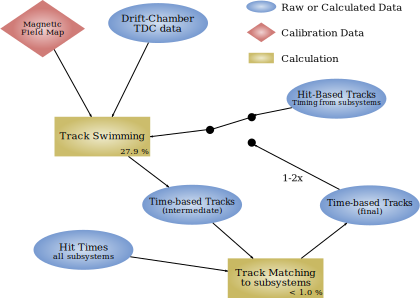
\includegraphics[width=0.8\columnwidth]{\figures/reconstruction/clas6_timebasedtracking_diagram_color.pdf}
\caption[Flow chart of the time-based tracking part of the reconstruction]{\label{fig:data.cook.flowchart.timebased}Flow chart of the time-based tracking part of the reconstruction shown in Fig.\ref{fig:data.cook.flowchart}. ``Subsystems'' refers to the \abbr{ST}, \abbr{CC}, \abbr{TOF} and the \abbr{EC} detectors. The switch indicates that hit-based tracks are input into the swimming calculation, after which the time-based tracks are used creating a feedback loop. Percentages shown indicate the relative time taken to do the calculations with respect to the full reconstruction.}
\end{center}\end{figure}




%The tagger energy was calibrated using the exclusive reaction:
%\begin{align}\label{rxn:excl_ppippim}
%    \mathrm{\gamma p \rightarrow p \pi^+ \pi^-}
%\end{align}
%where the exclusivity was determined via missing momentum and missing mass cuts using the energy of the tagger hit associated with the event. The photon energy was then adjusted by taking the total energy of the $\mathrm{p \pi^+ \pi^-}$ system using the equation:
%\begin{align}\label{eqn:ebeam_ppippim}
%    E_\mathrm{beam, corrected} = E_\p + E_{\mathrm{\pi^+}} + E_{\mathrm{\pi^-}} - m_\p,   
%\end{align}
%where $E_\p$, $E_{\mathrm{\pi^+}}$ and $E_{\mathrm{\pi^-}}$ are the energies of the outgoing particles, and $m_\p$ is the proton (target) mass. The average of at least 10k events per \emph{logical} tagger energy paddle (see Sec.~\ref{sec:clas.tagr}) was used for this correction and the results as a function of the beam energy is shown in Fig.~\ref{fig:data.calib.tag_energy}. The inherent resolution of the tagger paddles for \g12 was approximately 5.6~MeV.
%
%Results from the tagger energy calibration were used to calculate corrections to the momenta of the tracks, the energy corrections were subsequently recalculated. This iterative process was employed several times until the values obtained for both corrections converged. The energy difference between $E_\mathrm{beam, corrected}$ in Eq.~\ref{eqn:ebeam_ppippim} and the energy reported by the tagger is shown in Fig.~\ref{fig:data.calib.ediff_ppippim}.
%
%The resolution of the tagger time is approximately 130~ps as shown in Fig.~\ref{fig:data.calib.dttag_ppippim} and this value is used to identify the \abbr{RF} beam-bucket associated with the event. The \abbr{RF} provides the best timing resolution, on the order of a few picoseconds, in \abbr{CLAS} and it is used to calibrate the other systems as described in the sections below.

\section{Particle Identification}\label{sec:data.pid}

The final procedure is to assign the track a particle mass ($m$). In Sec.~\ref{sec:clas.tof} Eqs.~\ref{eq:beta.cal} and~\ref{eq:mass.cal} explain how the mass of a particle is determined. Fig.~\ref{fig:data.pid} depicts a 2-dimensional plot of the quantities used to determine the particle mass. Once the mass has been determined, particle identification \abbr{PID} is determined by the following criteria;
%Figure~\ref{fig:data.pid} depicts a plot of the quantities used to determine the particles mass,
\begin{align}\label{list:pid}
\abbr{PID} =
\begin{cases}
\pi^{\pm}, & \mathrm{if} \  m  <  0.3~\mathrm{GeV} \ \mathrm{and} \  q  \pm \\
K^{\pm}, &  \mathrm{if} \ 0.35 < m  <  0.35~\mathrm{GeV} \ \mathrm{and} \  q  \pm  \\
p^{\pm}, & \mathrm{if \ 0.8 \ < \ }m \mathrm{\ < \ 1.2 \ GeV \  and \  q  \pm} \\
d, & \mathrm{if \ 1.75 \ < \  }m  \mathrm{\ < \ 2.2 \ GeV } \\
\end{cases}
\end{align}
The events which had particles falling within the undefined regions of the cuts listed in Eq.~\ref{list:pid} were deemed ambiguous events and were given the \abbr{PID} of \emph{``unknown''}. For the analysis of this work, \emph{``unknown''} were used and is described in Sec.~\ref{sec:analysis}

Since tracking began after the particle had already traversed through the target and \abbr{ST}, the measured momentum determination was decreased by the ``energy-loss'' the particle underwent before entering the Region 1 \abbr{DC}. These effects were taken into account as part of the ``energy-loss'' correction during the analysis phase as discussed in Sec.~\ref{sec:analysis.corrections.eloss}.  Once particle identification is completed on the reconstruction level, all relevant information about the particle is collected into the event of occurrence and this information is written in \abbr{BOS} format. There are multiple methods for analyzing \abbr{BOS} format, the chapter~\ref{sec:analysis} will discuss the method used in this analysis. 
%
\begin{figure}\begin{center}
\includegraphics[width=0.9\columnwidth,height=\hfigheight]{\figures/hall-b/g12_pid.pdf}
\caption[$\beta$ vs. mometum(p)$\times$charge(q) for run 56855]{\label{fig:data.pid} $\beta$ vs. mometum(p)$\times$charge(q) for run 56855. This plot is a graphical representation of how particle ID assignments are made in CLAS reconstruction. The ``ribs" seen represent tracks that were ``out-of-time" with a incident photon. Image Source:~\cite{bookwalter}}
\end{center}\end{figure}
